\chapter{Twierdzenia o wartości średniej}
\label{ma2:ch:mean-value}

W tym rozdziale $E,F$ są rzeczywistymi przestrzeniami
Banacha, $U\subseteq E$ jest otwarty, a $[x,y]$ oznacza
odcinek $\{x+t(y-x):0\le t\le1\}$.
Pochodna oznacza pochodną Frécheta, o ile nie
zaznaczono inaczej. Podstawową metodą jest badanie
funkcji jednej zmiennej na odcinkach. W szczególności
nie zakładamy zwartości kul w przestrzeni Banacha.

\section{Skalarne twierdzenia o wartości średniej}

\begin{twierdzenie}[Lagrange'a i Rolle'a na odcinku]
\label{ma2:thm:scalar-mvt}
Niech $f:U\to\R$, $x,y\in U$, $x\ne y$, $[x,y]\subseteq U$.
Załóżmy, że $f$ jest ciągła na odcinku i różniczkowalna
w każdym punkcie odcinka poza jego końcami
(tj. dla parametrów $t\in(0,1)$). Istnieje $\theta\in(0,1)$ takie, że
\[
 f(y)-f(x)=Df(x+\theta(y-x))(y-x).
\]
Jeśli $f(x)=f(y)$, prawa strona jest zerowa.
\end{twierdzenie}
\begin{proof}
Funkcja $\gamma(t)=f(x+t(y-x))$ jest ciągła na $[0,1]$,
a odwzorowanie $t\mapsto x+t(y-x)$ jest afiniczne
i ma pochodną $s\mapsto s(y-x)$. Z twierdzenia
\ref{ma2:thm:frechet-chain} funkcja $\gamma$ ma
pochodną $\gamma'(t)=Df(x+t(y-x))(y-x)$ dla $0<t<1$.
Twierdzenie Lagrange'a (AM I 21.3.1), zastosowane do
$\gamma$, daje tezę. Jeśli wartości końcowe są równe,
otrzymujemy wersję Rolle'a (por. AM I 21.2.1).
\end{proof}

W wersji Rolle'a nie wynika, że $Df$ jest operatorem
zerowym w punkcie pośrednim. Przykładowo
$f(s,t)=t$ dla $x=(0,0)$ i $y=(1,0)$ ma równe
wartości na końcach odcinka, ale $Df(s,t)(h,k)=k$
w każdym punkcie.

\begin{wniosek}[Cauchy'ego na odcinku]
\label{ma2:cor:scalar-cauchy}
Jeżeli funkcje $f,g:U\to\R$ spełniają założenia
twierdzenia \ref{ma2:thm:scalar-mvt} dla tych samych
$x,y$, to istnieje $z=x+\theta(y-x)$, $0<\theta<1$,
dla którego
\[
 (f(y)-f(x))Dg(z)(y-x)
 =(g(y)-g(x))Df(z)(y-x).
\]
Jeżeli $Dg(x+t(y-x))(y-x)\ne0$ dla każdego $t\in(0,1)$,
to $g(y)\ne g(x)$ i można podzielić równość przez
$(g(y)-g(x))Dg(z)(y-x)$.
\end{wniosek}
\begin{proof}
Stosujemy AM I 21.4.1--2 do przekrojów $f$ i $g$
na odcinku, których pochodne wyznacza reguła
łańcuchowa jak w poprzednim dowodzie.
\end{proof}

\section{Nierówność dla odwzorowań wektorowych}

\begin{twierdzenie}[Oszacowanie przyrostu]
\label{ma2:thm:mean-value-inequality}
Niech $f:U\to F$ będzie ciągłe na $[x,y]\subseteq U$
i różniczkowalne w punktach odcinka poza jego końcami.
Jeżeli $x\ne y$ i $\|Df(x+t(y-x))\|\le M$ dla
$t\in(0,1)$, gdzie $M\ge0$, to
\[
 \|f(y)-f(x)\|\le M\|y-x\|.
\]
\end{twierdzenie}
\begin{proof}
Dla $\gamma(t)=f(x+t(y-x))$ reguła łańcuchowa daje
$\|\gamma'(t)\|\le M\|y-x\|$.
Stosujemy lemat \ref{ma2:lem:vector-increment}
na $[0,1]$. Dla $x=y$ analogiczna nierówność jest
trywialna. Dowód działa także w przestrzeniach
unormowanych, gdyż przywołany lemat nie wymaga
zupełności. Wystarczy nawet bezpośrednie oszacowanie
$\|Df(x+t(y-x))(y-x)\|\le M\|y-x\|$:
ograniczenie normy całego operatora nie jest konieczne.
\end{proof}

\begin{przyklad}[Brak wektorowej równości Lagrange'a]
\label{ma2:ex:vector-mvt-failure}
Krzywa $\gamma:\R\to\R^2$ dana przez
$\gamma(t)=(\cos t,\sin t)$ spełnia
$\gamma(2\pi)=\gamma(0)$. Jednak
$\gamma'(t)=(-\sin t,\cos t)$ ma normę $1$ w każdym
punkcie. Nie istnieje zatem $c\in(0,2\pi)$ takie,
że $\gamma(2\pi)-\gamma(0)=2\pi\gamma'(c)$.
Nie zachodzi również wektorowa wersja twierdzenia
Rolle'a z zerową pochodną.
\end{przyklad}

\begin{figure}[htbp]
\centering
\begin{tikzpicture}[x=1.65cm,y=1.65cm,>=Stealth]
 \draw[->,gray] (-1.65,0)--(2.15,0) node[right] {$x_1$};
 \draw[->,gray] (0,-1.45)--(0,1.5) node[above] {$x_2$};
 \draw[blue!70!black,thick] (0,0) circle[radius=1];
 \fill (1,0) circle (1.6pt);
 \node[anchor=west,xshift=4pt,yshift=8pt] at (1,0) {$P$};
 \coordinate (Q) at ({cos(45)},{sin(45)});
 \fill (Q) circle (1.6pt);
 \draw[->,red!70!black,very thick] (Q)--++(-.7071,.7071);
 \node[anchor=west,xshift=5pt,yshift=1pt] at (Q) {$Q$};
 \node[red!70!black,anchor=east,xshift=-8pt] at (-.12,1.36) {$v$};
 \draw[->,blue!70!black,thick] ({cos(200)},{sin(200)})
  arc[start angle=200,end angle=245,radius=1];
\end{tikzpicture}
\caption{Krzywa jednostkowa wraca do punktu $P=\gamma(0)=
\gamma(2\pi)$, lecz jej wektor styczny nigdy nie jest zerowy.
W punkcie $Q=\gamma(\pi/4)$ zaznaczono wektor
$v=\gamma'(\pi/4)$, styczny do okręgu.}
\label{ma2:fig:vector-mvt-failure}
\end{figure}
\FloatBarrier

\subsection{Bezpośredni dowód w przestrzeni euklidesowej}

Dla $E=\R^n$, $F=\R^m$ z normami euklidesowymi
można udowodnić twierdzenie
\ref{ma2:thm:mean-value-inequality} bez twierdzenia
Hahna--Banacha. Jeśli $w=f(y)-f(x)\ne0$, rozważmy
funkcję skalarną
\[
 \varphi(t)=\left\langle f(x+t(y-x)),\frac{w}{\|w\|_2}
                         \right\rangle.
\]
Funkcjonał $u\mapsto\langle u,w/\|w\|_2\rangle$
jest liniowy i ciągły z nierówności
Cauchy'ego--Schwarza. Zatem $\varphi$ jest ciągła
na $[0,1]$, a z reguły łańcuchowej
\[
 \varphi'(t)=
 \left\langle Df(x+t(y-x))(y-x),w/\|w\|_2\right\rangle
 \quad(0<t<1).
\]
Ponieważ
$\varphi(1)-\varphi(0)=\|w\|_2$, twierdzenie Lagrange'a
i nierówność Cauchy'ego--Schwarza dają dla pewnego
$\theta\in(0,1)$
\[
 \|w\|_2=\varphi'(\theta)
 \le \|Df(x+\theta(y-x))(y-x)\|_2
 \le M\|y-x\|_2 .
\]
Dla $w=0$ teza jest oczywista. Ten dowód wykorzystuje
rzut przyrostu na jego własny kierunek. W ogólnej
przestrzeni Banacha rolę iloczynu skalarnego z
jednostkowym wektorem pełni funkcjonał normujący
(por. dowód lematu \ref{ma2:lem:vector-increment}).
Osobne stosowanie twierdzenia Lagrange'a do każdej
współrzędnej nie daje na ogół wspólnego punktu
pośredniego.

\section{Całkowa reprezentacja przyrostu}

Korzystamy z definicji całki Riemanna o wartościach
wektorowych z rozdziału \ref{ma2:ch:limits-calculus}.
Poniższy lemat i twierdzenie przytaczamy z analizy
funkcjonalnej (AF 14.19--20), bez powielania dowodów.

\begin{lemat}[Podstawowe twierdzenie rachunku dla krzywych]
\label{ma2:lem:ftc-banach}
Jeżeli $\gamma:[a,b]\to F$ jest klasy $C^1$,
$a<b$ (pochodne na końcach są jednostronne, a
pochodna jest ciągła na $[a,b]$), to $\gamma'$ jest
całkowalna w sensie Riemanna z wartościami w $F$ i
\[
 \gamma(b)-\gamma(a)=\int_a^b\gamma'(t)\,\mathrm dt.
\]
\end{lemat}
\emph{Dowód:} AF 14.19 (\texttt{lem:ftc-banach14}).
W dowodzie istnienie całki wynika z jednostajnej
ciągłości $\gamma'$ i zupełności $F$, a równość z
sumowania przyrostów oszacowanych przez moduł
ciągłości pochodnej.

\begin{twierdzenie}[Wzór całkowy na przyrost]
\label{ma2:thm:integral-increment}
Niech $f\in C^1(U,F)$ oraz $[x,y]\subseteq U$.
Wówczas
\[
 f(y)-f(x)=\int_0^1 Df(x+t(y-x))(y-x)\,\mathrm dt
\]
oraz
\[
 \|f(y)-f(x)\|\le
 \|y-x\|\int_0^1\|Df(x+t(y-x))\|\,\mathrm dt.
\]
\end{twierdzenie}
\emph{Dowód:} AF 14.20 (\texttt{thm:mean-value14}).
Dla pierwszej równości stosuje się lemat
\ref{ma2:lem:ftc-banach} do przekroju odcinkowego
oraz regułę łańcuchową. Druga nierówność wynika
z nierówności dla normy całki: dla ciągłej
$g:[0,1]\to F$ suma Riemanna spełnia
$\|R(g,P)\|\le R(\|g\|,P)$, a obie strony mają granice
przy średnicy podziału dążącej do zera. Następnie
stosujemy definicję normy operatorowej.
Nie utożsamiamy wzoru całkowego z równością
Lagrange'a w pojedynczym punkcie.

\begin{przyklad}
Dla algebry Banacha $A$ i $P:A\to A$, $P(x)=x^2$,
mamy $DP(x)h=xh+hx$ (twierdzenie
\ref{ma2:thm:frechet-bilinear}).
Dla $y=x+h$ wzór całkowy daje
\[
 \begin{aligned}
 P(x+h)-P(x)
 &=\int_0^1 ((x+th)h+h(x+th))\,\mathrm dt\\
 &=xh+hx+h^2 .
 \end{aligned}
\]
Pochodna jest ciągła w normie operatorowej, ponieważ
dla $\|k\|\le1$ podmultiplikatywność normy daje
$\|(DP(x)-DP(y))k\|
=\|(x-y)k+k(x-y)\|\le2\|x-y\|$.
Po supremum po takich $k$ otrzymujemy
$\|DP(x)-DP(y)\|\le2\|x-y\|$. W obliczeniu całki
korzystamy z liniowości sum Riemanna, ciągłości
odwzorowania skalarów w wielokrotności ustalonego wektora i $\int_0^1t\,\mathrm dt=1/2$.
Nie zakładamy przemienności algebry.
\end{przyklad}

\section{Warunki Lipschitza i oszacowanie reszty}

\begin{wniosek}
\label{ma2:cor:derivative-lipschitz}
Niech $V\subseteq U$ będzie niepustym zbiorem wypukłym,
a $f:U\to F$ różniczkowalne na $V$. Jeżeli
$\sup_{z\in V}\|Df(z)\|\le M<\infty$, to $f$ jest
funkcją Lipschitza na $V$ ze stałą $M$.
Jeżeli $f\in C^1(U,F)$, to $f$ jest lokalnie funkcją
Lipschitza w każdym punkcie $U$.
\end{wniosek}
\begin{proof}
Pierwsza teza wynika z twierdzenia
\ref{ma2:thm:mean-value-inequality} na każdym odcinku
$[x,y]\subseteq V$. Dla $p\in U$ z otwartości $U$
i ciągłości $Df$ wybieramy $r>0$ tak, że
$B(p,r)\subseteq U$ i $\|Df(z)-Df(p)\|\le1$
dla $z\in B(p,r)$. Kula jest wypukła, a
$\|Df(z)\|\le\|Df(p)\|+1$, więc stosujemy pierwszą tezę.
Nie korzystamy ze zwartości kuli.
\end{proof}

\begin{stwierdzenie}[Oszacowanie pochodnej funkcji Lipschitza]
\label{ma2:prop:lipschitz-derivative}
Jeśli $f$ jest funkcją Lipschitza ze stałą $L$ na
otoczeniu punktu $p\in U$ i ma w $p$ pochodną
Frécheta, to $\|Df(p)\|\le L$.
\end{stwierdzenie}
\begin{proof}
Dla $h\in E$ i niezerowego rzeczywistego $t$ o
dostatecznie małym module punkty $p,p+th$ należą
do tego otoczenia. Stąd
\[
 \left\|\frac{f(p+th)-f(p)}{t}\right\|\le L\|h\|.
\]
Na mocy twierdzenia \ref{ma2:thm:frechet-gateaux}
iloraz wektorowy dąży do $Df(p)h$. Przechodząc
do granicy norm i biorąc supremum po $\|h\|\le1$,
otrzymujemy tezę.
\end{proof}

Założenia wypukłości w poprzednim wniosku nie można
po prostu pominąć. Na zbiorze otwartym
$U=(-1,0)\cup(0,1)\subseteq\R$ funkcja równa $0$
na pierwszej składowej i $1$ na drugiej ma wszędzie
pochodną zerową, ale nie jest funkcją Lipschitza na
całym $U$: dla $x=-1/n$, $y=1/n$, $n\ge2$,
iloraz $|f(y)-f(x)|/|y-x|$ wynosi $n/2$.
Nawet spójność zbioru nie zastępuje wypukłości
w ogólnym oszacowaniu Lipschitza, jak pokazuje
następny przykład.

\begin{przyklad}[Spójny obszar nie wystarcza]
\label{ma2:ex:connected-nonconvex-lipschitz}
Niech
\[
 V=(-2,2)^2\setminus\{(s,0):s\ge0\}.
\]
Jest to zbiór otwarty, ponieważ usunięta półprosta
jest domknięta w $\R^2$. Jest on spójny, a nawet
łukowo spójny: każdy punkt z niezerową drugą
współrzędną można połączyć poziomym odcinkiem
z prostą $x=-1$, a następnie pionowym odcinkiem
z punktem $(-1,0)$. Dla punktów o zerowej drugiej
współrzędnej mamy $x<0$ i wystarczy odcinek poziomy.
Zdefiniujmy $f:V\to\R$ przez
\[
 f(x,y)=
 \begin{cases}
  (\max\{x,0\})^2,&y>0,\\
  0,&y\le0.
 \end{cases}
\]
Funkcja jednej zmiennej $s\mapsto(\max\{s,0\})^2$
jest klasy $C^1$: jej pochodna to $2\max\{s,0\}$,
także w zerze, gdzie iloraz różnicowy ma moduł
nie większy niż $|s|$. W górnej części $V$ mamy
zatem $Df(x,y)(h,k)=2\max\{x,0\}h$.
W dolnej części $V$ pochodna jest zerowa.
Jeżeli $(x,0)\in V$, to $x<0$ i w pewnym
otoczeniu tego punktu $f$ jest identycznie zerowa.
Wynika stąd, że $f\in C^1(V,\R)$ i
$\|Df(x,y)\|\le4$ w normie euklidesowej.
Jednak dla $p_n=(1,1/n)$ i $q_n=(1,-1/n)$,
$n\ge1$, mamy
\[
 |f(p_n)-f(q_n)|=1,\qquad
 \|p_n-q_n\|_2=\frac2n.
\]
Iloraz przyrostów wynosi $n/2$ i nie jest ograniczony.
Zatem $f$ nie jest funkcją Lipschitza na $V$,
mimo że $V$ jest spójny, a pochodna jest ograniczona.
Odcinek $[p_n,q_n]$ przecina usuniętą półprostą,
więc twierdzenia o oszacowaniu przyrostu nie można
do niego zastosować.
\end{przyklad}

W następnym wniosku spójność wystarczy jednak
do stałości funkcji o zerowej pochodnej.

\begin{wniosek}
\label{ma2:cor:zero-derivative}
Niech $f:U\to F$ będzie różniczkowalne na $U$.
Jeżeli $U$ jest spójny i $Df=0$ na $U$, to
$f(x)=f(y)$ dla wszystkich $x,y\in U$.
\end{wniosek}
\begin{proof}
W każdej dostatecznie małej kuli zawartej w $U$
poprzedni wniosek ze stałą $M=0$ daje stałość $f$.
Jeżeli $U$ jest niepusty i $p\in U$, to zbiór
$\{x\in U:f(x)=f(p)\}$ oraz jego dopełnienie są
otwarte w $U$, ponieważ $f$ jest lokalnie stałe.
Ze spójności i niepustości tego zbioru wynika,
że jest on równy $U$.
\end{proof}

\begin{twierdzenie}[Oszacowanie względem ustalonego operatora]
\label{ma2:thm:linear-approximation-bound}
Niech $V\subseteq U$ będzie niepustym zbiorem wypukłym,
$f:U\to F$ różniczkowalne na $V$ i $A\in\mathcal L(E,F)$. Jeżeli
$\sup_{z\in V}\|Df(z)-A\|\le q$, $q\ge0$, to dla
wszystkich $x,y\in V$ zachodzi
\[
 \|f(y)-f(x)-A(y-x)\|\le q\|y-x\|.
\]
\end{twierdzenie}
\begin{proof}
Stosujemy wniosek \ref{ma2:cor:derivative-lipschitz}
do odwzorowania $g(z)=f(z)-Az$, którego pochodna
wynosi $Df(z)-A$ na mocy twierdzenia
\ref{ma2:thm:frechet-chain}.
\end{proof}

\begin{wniosek}[Dolne oszacowanie przyrostu]
\label{ma2:cor:lower-increment}
Przy założeniach poprzedniego twierdzenia, jeżeli
$\|Ah\|\ge m\|h\|$ dla każdego $h\in E$, gdzie $m>q$,
to
\[
 (m-q)\|y-x\|\le\|f(y)-f(x)\|
 \le(\|A\|+q)\|y-x\|\qquad(x,y\in V).
\]
W szczególności $f|_V$ jest różnowartościowe, a jego
odwrotność na $f(V)$ jest funkcją Lipschitza ze
stałą $1/(m-q)$.
\end{wniosek}
\begin{proof}
Zapisujemy $f(y)-f(x)=A(y-x)+r$, gdzie
$\|r\|\le q\|y-x\|$. Nierówność trójkąta i jej
odwrotna postać dają odpowiednio oszacowania z góry
i z dołu. Dla $x\ne y$ dolne oszacowanie jest
dodatnie, co daje różnowartościowość. Po podzieleniu
przez $m-q$ otrzymujemy nierówność dla odwrotności.
\end{proof}

Niech $p\in U$, $E,F\ne\{0\}$ i niech $f$ będzie
różniczkowalne w otoczeniu $p$, a $Df$ ciągłe w $p$.
Jeżeli $A=Df(p)$ jest izomorfizmem przestrzeni Banacha,
to $\|h\|=\|A^{-1}Ah\|\le\|A^{-1}\|\|Ah\|$.
Możemy zatem przyjąć $m=\|A^{-1}\|^{-1}>0$.
Wybierając $q=m/2$ i dostatecznie małą kulę wokół
$p$, z ciągłości $Df$ w $p$ zapewniamy
$\|Df(z)-A\|\le q$ na tej kuli. Otrzymaliśmy lokalną
różnowartościowość, ale nie udowodniliśmy jeszcze
otwartości obrazu ani różniczkowalności odwrotności.
Te kwestie rozstrzygniemy w twierdzeniu o funkcji
odwrotnej.

\begin{przyklad}
Niech $f:\R^2\to\R^2$, $f(x,y)=(x+y^2,y+x^2)$.
Dla $z=(x,y)$ w normie euklidesowej
\[
 Df(z)-I=\begin{pmatrix}0&2y\\2x&0\end{pmatrix},
 \qquad \|Df(z)-I\|=2\max(|x|,|y|).
\]
Istotnie, kwadrat normy obrazu $(h,k)$ przez tę
macierz wynosi $4y^2k^2+4x^2h^2$; maksimum na
sferze jednostkowej otrzymujemy na jednej z osi.
Na kuli $B(0,1/4)$ norma różnicy jest co najwyżej
$1/2$. Dla $A=I$ mamy $m=1$, zatem
\[
 \tfrac12\|z-w\|_2\le\|f(z)-f(w)\|_2
 \le\tfrac32\|z-w\|_2
 \qquad(z,w\in B(0,1/4)).
\]
W szczególności $f$ jest różnowartościowe na tej kuli.
\end{przyklad}

\begin{wniosek}[Kwadratowe oszacowanie reszty]
\label{ma2:cor:quadratic-remainder}
Niech $f\in C^1(U,F)$, $p,p+h\in U$ i
$[p,p+h]\subseteq U$. Załóżmy, że $L\ge0$ oraz
$\|Df(p+th)-Df(p)\|\le Lt\|h\|$ dla $0\le t\le1$.
W szczególności warunek ten zachodzi, gdy $Df$ jest
funkcją Lipschitza ze stałą $L$ na odcinku. Wtedy
\[
 \|f(p+h)-f(p)-Df(p)h\|
 \le \frac L2\|h\|^2.
\]
\end{wniosek}
\begin{proof}
Wzór z twierdzenia \ref{ma2:thm:integral-increment}
oraz liniowość całki dają
\[
 f(p+h)-f(p)-Df(p)h
 =\int_0^1 (Df(p+th)-Df(p))h\,\mathrm dt.
\]
Norma funkcji podcałkowej jest oszacowana przez
$Lt\|h\|^2$. Z nierówności dla normy całki i
$\int_0^1 t\,\mathrm dt=1/2$ otrzymujemy tezę,
również dla $h=0$.
\end{proof}
Stała $1/2$ jest optymalna: dla $f(s)=Ls^2/2$,
$L>0$, $p=0$ na $\R$ pochodna jest funkcją Lipschitza
ze stałą $L$, a w oszacowaniu zachodzi równość.

\paragraph{Rysunek 3D: Kwadratowe oszacowanie reszty.}
Dla $f(x,y)=x^2+2y^2$ mamy $Df(0)=0$ oraz
$\|Df(h)-Df(k)\|_2\le4\|h-k\|_2$, ponieważ
gradient przyrostu ma współrzędne $2(h_1-k_1)$
i $4(h_2-k_2)$. Wniosek \ref{ma2:cor:quadratic-remainder}
daje $0\le f(x,y)\le2(x^2+y^2)$. Porównujemy resztę
z jej górnym ograniczeniem; na osi $y$ zachodzi równość.
Kod wymaga bibliotek NumPy i Plotly; zapisuje samodzielny
interaktywny plik HTML.
Rysunek \ref{ma2:fig:quadratic-remainder-surfaces} przedstawia wersję statyczną.

\begin{figure}[htbp]
\centering
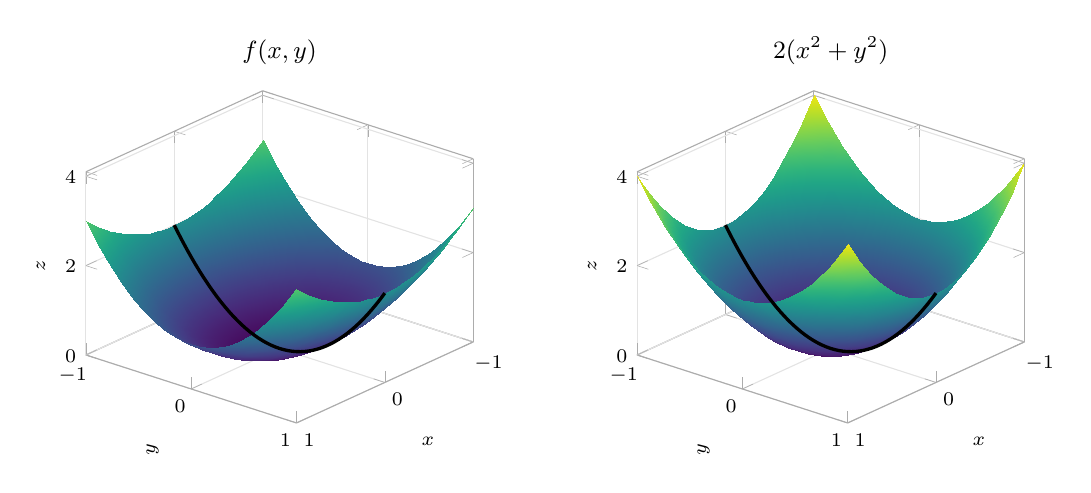
\begin{tikzpicture}
\begin{scope}[xshift=0cm]
\begin{axis}[width=6.5cm,height=5.8cm,view={130}{30},axis lines=box,grid=major,major grid style={draw=gray!22},axis line style={gray!65},tick style={gray!65},
xmin=-1,xmax=1,ymin=-1,ymax=1,zmin=0,zmax=4.1,
xtick={-1,0,1},ytick={-1,0,1},tick label style={font=\scriptsize},
xlabel=$x$,ylabel=$y$,zlabel=$z$,label style={font=\scriptsize},
title={$f(x,y)$},title style={font=\small},
colormap name=viridis,point meta min=0,point meta max=4.1]
\addplot3[surf,shader=interp,draw=none,z buffer=sort,domain=-1:1,domain y=-1:1,samples=31,samples y=31] {x^2+2*y^2};
\addplot3[very thick,black,domain=-1:1,samples=51,samples y=1] (0,x,2*x^2);
\end{axis}
\end{scope}
\begin{scope}[xshift=7cm]
\begin{axis}[width=6.5cm,height=5.8cm,view={130}{30},axis lines=box,grid=major,major grid style={draw=gray!22},axis line style={gray!65},tick style={gray!65},
xmin=-1,xmax=1,ymin=-1,ymax=1,zmin=0,zmax=4.1,
xtick={-1,0,1},ytick={-1,0,1},tick label style={font=\scriptsize},
xlabel=$x$,ylabel=$y$,zlabel=$z$,label style={font=\scriptsize},
title={$2(x^2+y^2)$},title style={font=\small},
colormap name=viridis,point meta min=0,point meta max=4.1]
\addplot3[surf,shader=interp,draw=none,z buffer=sort,domain=-1:1,domain y=-1:1,samples=31,samples y=31] {2*(x^2+y^2)};
\addplot3[very thick,black,domain=-1:1,samples=51,samples y=1] (0,x,2*x^2);
\end{axis}
\end{scope}
\end{tikzpicture}
\caption{Reszta $x^2+2y^2$ i jej ograniczenie $2(x^2+y^2)$ we wspólnej skali. Czarna krzywa w obu panelach odpowiada równości na osi $x=0$.}
\label{ma2:fig:quadratic-remainder-surfaces}
\end{figure}

\begin{lstlisting}[language=Python]
import numpy as np
import plotly.graph_objects as go

x = np.linspace(-1, 1, 81)
X, Y = np.meshgrid(x, x)
fig = go.Figure()
for z, name, color in [(X**2+2*Y**2, "reszta", "Blues"),
                      (2*(X**2+Y**2), "ograniczenie",
                       "Oranges")]:
    fig.add_trace(go.Surface(x=X, y=Y, z=z,
        opacity=0.65, name=name, colorscale=color,
        showscale=False, showlegend=True))
fig.update_layout(scene=dict(xaxis_title="x",
    yaxis_title="y", zaxis_title="z"))
fig.write_html("am2_14_remainder.html", include_plotlyjs=True)
fig.show()
\end{lstlisting}

\section{Ciągłość pochodnej Gâteaux}

\begin{twierdzenie}[Ciągła pochodna Gâteaux]
\label{ma2:thm:continuous-gateaux}
Jeżeli $f:U\to F$ jest różniczkowalne w sensie
Gâteaux w każdym punkcie $U$ i
$D_Gf:U\to\mathcal L(E,F)$ jest ciągłe w normie
operatorowej, to $f\in C^1(U,F)$ oraz $Df=D_Gf$.
\end{twierdzenie}
\emph{Dowód:} AF 14.21 (\texttt{thm:continuous-gateaux14}).
Dla przekroju $\gamma(t)=f(p+th)$ pochodna istnieje
z definicji pochodnej kierunkowej, a ciągłość
$D_Gf$ zapewnia ciągłość $\gamma'$.
Lemat \ref{ma2:lem:ftc-banach} pozwala wyrazić
przyrost przez całkę; oszacowanie reszty przez
$\|h\|\sup_{0\le t\le1}\|D_Gf(p+th)-D_Gf(p)\|$
daje różniczkowalność Frécheta.

\begin{wniosek}[Wystarcza ciągłość w rozważanym punkcie]
\label{ma2:cor:pointwise-gateaux}
Niech $f:U\to F$ i $p\in U$.
Jeżeli $D_Gf$ istnieje w otoczeniu $p$ i jest
ciągłe w $p$ w normie operatorowej, to $Df(p)$
istnieje i $Df(p)=D_Gf(p)$.
\end{wniosek}
\begin{proof}
Niech $A=D_Gf(p)$. Dla $\varepsilon>0$ wybieramy
$\delta>0$ tak, że $B(p,\delta)\subseteq U$,
pochodne Gâteaux istnieją w tej kuli i
$\|D_Gf(z)-A\|\le\varepsilon$ w tej kuli.
Dla $\|h\|<\delta$ rozważamy
$\gamma(t)=f(p+th)-tAh$ na $[0,1]$.
Jeśli $h=0$, żądana nierówność dla reszty jest
trywialna. Dla $h\ne0$ oraz $t\in[0,1]$ punkt
$z=p+th$ leży w otwartej kuli $B(p,\delta)$.
Dla dostatecznie małych $s\ne0$ także $z+sh$
leży w tej kuli, a z definicji pochodnej Gâteaux
\[
 \frac{\gamma(t+s)-\gamma(t)}{s}
 =\frac{f(z+sh)-f(z)}{s}-Ah
 \longrightarrow (D_Gf(z)-A)h.
\]
Na końcach odcinka wystarczy brać jednostronne
przyrosty parametru. Istnienie tych pochodnych
zapewnia ciągłość $\gamma$ na $[0,1]$.
Dla $0<t<1$ mamy
\[
 \gamma'(t)=(D_Gf(p+th)-A)h,\qquad
 \|\gamma'(t)\|\le\varepsilon\|h\|.
\]
Lemat \ref{ma2:lem:vector-increment} daje
$\|f(p+h)-f(p)-Ah\|\le\varepsilon\|h\|$.
Z dowolności $\varepsilon$ wynika teza. W tym
dowodzie nie używamy całki ani zupełności.
\end{proof}

Ciągłość $D_Gf$ w normie operatorowej oznacza
jednostajną kontrolę względem $\|h\|\le1$:
$\sup_{\|h\|\le1}\|(D_Gf(z)-D_Gf(p))h\|\to0$
dla $z\to p$. Nie zastępujemy jej samą ciągłością
przekrojów funkcji $f$ na prostych. Przykład
\ref{ma2:ex:frechet-counterexample} przypomina, że
samo istnienie pochodnej Gâteaux w punkcie i
ciągłość funkcji nie zapewniają różniczkowalności
Frécheta.

W dalszym ciągu wykorzystamy oszacowania przyrostów
dla odwzorowań o wartościach operatorowych, badając
pochodne wyższych rzędów i wzory Taylora.
